\chapter{La rete cellulare}
La rete cellulare è la struttura \textit{hardware} e \textit{software} che consente il corretto
funzionamento delle comunicazioni tramite i dispositivi cellulari, dalle normali comunicazioni vocali alle \textit{smart cities} nel 5G.\\
Grazie ad una fitta rete di antenne, i gestori telefonici riescono a garantire il servizio per la  gran parte del territorio mondiale.
\begin{figure}[h]
    \centering
    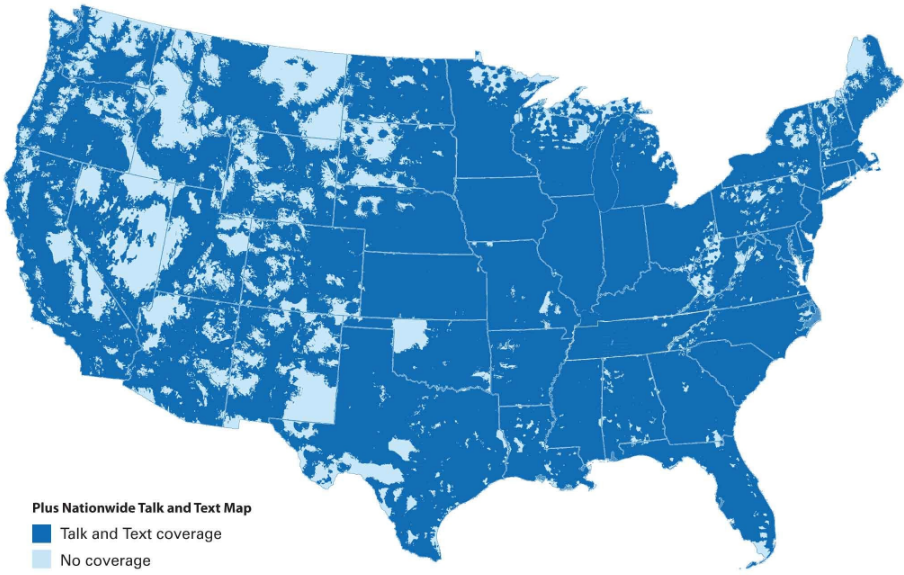
\includegraphics[width=0.7\textwidth]{images/att-coverage.png}
    \caption{Mappa compertura AT\&T negli USA}
\end{figure}\\

\clearpage

\section{Struttura}
La loro struttura e architectura hanno subito numerosi cambiamenti nel corso delle generazioni, in particolare con la rete
5G.\\
Si possono comunque identificare degli elementi chiave che sono presenti in tutte le generazioni:
\begin{itemize}
    \item \gls{ms} ovvero il dispositivo cellulare, in alcune generazioni questo acronimo è leggermente diverso, come per esempio dal 3G è
    lo \gls{ue}.
    \item \gls{ran} ovvero l'infrastruttura fisica di antenne per la ricezione e trasmissione di informazioni per il dispositivo
    \item \textit{Core Network} ovvero i componenti della sua architettura
\end{itemize}
\begin{figure}[h]
    \centering
    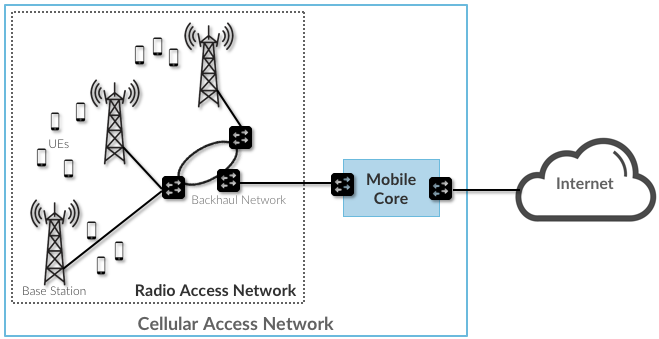
\includegraphics[width=0.9\textwidth]{images/cellular-network-basic-scheme.png}
    \caption{Schema di una rete cellulare}
\end{figure}

\clearpage

\noindent La \gls{ran} è composta ripetitori di segnale chiamati \gls{bs}. 
Questi vengono disposti in modo capillare sul territorio, suddividendolo in diverse aree di competenza chiamate celle. Ognuna di queste può gestire
un numero limitato di dispositivi in contemporanea, per questo, in caso di aree densamente popolate vengono 
ridotte le aree di competenza di ciascuna antenna. Le celle quindi, possono avere una dimensione variabile che dipende dal contesto in cui devono essere inserite.
\begin{figure}[h]
    \centering
    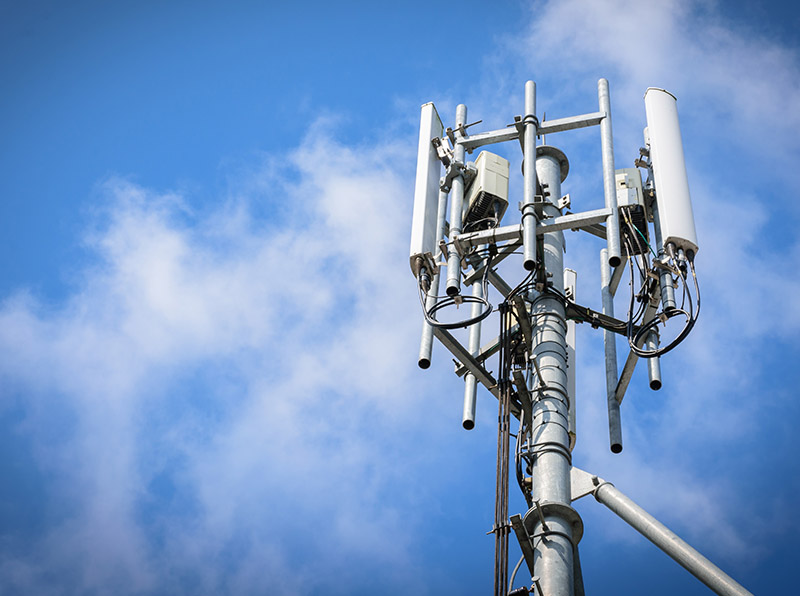
\includegraphics[width=0.5\textwidth]{images/base-station.jpg}
    \caption{\textit{Base Station}}
\end{figure}\\
Ogni cella ha un determinato raggio di azione che dipende dalle caratteristiche fisiche dell'antenna stessa. Inoltre, 
ha a disposizione un determinato range di frequenze su cui instaurare la comunicazione con i vari dispositivi, che solitamente
sono differenti rispetto a quelle usate dalle celle vicine per evitare interferenze.
Celle sufficientemente distanti possono utilizzare le stesse frequenze poiché non corrono il rischio di interferenza, questo rappresenta
un grande vantaggio per questa tecnologia.\\

\noindent Per identificare e autenticare ogni \gls{ms} nella rete è necessario che sia fornito del \gls{sim}, ossia una scheda fisica 
che contiene le chiavi per autenticarsi alla rete.
\begin{figure}[h]
    \centering
    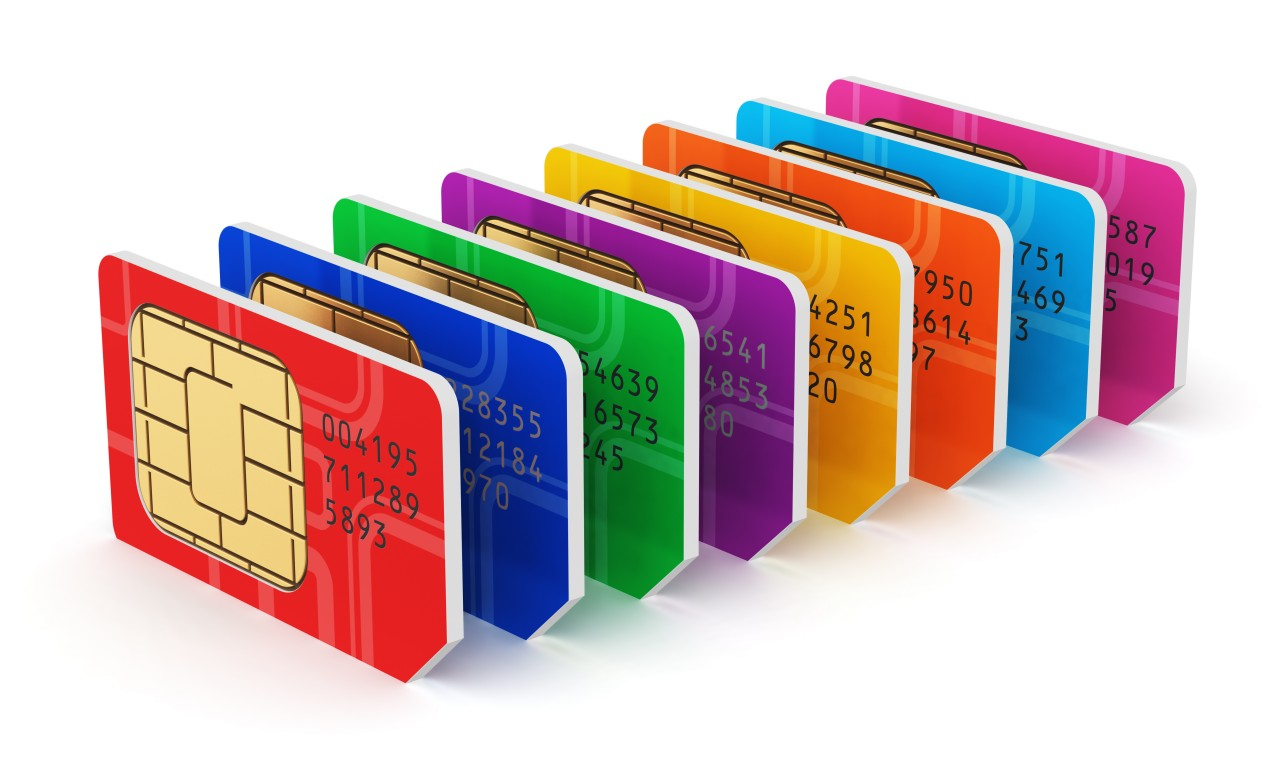
\includegraphics[width=0.5\textwidth]{images/simcard.jpg}
    \caption{\textit{Subscriber Identity Module}}
\end{figure}

\clearpage

\section{Architettura}
L'architettura di una rete cellulare è l'insieme dei componenti che permettono il suo corretto funzionamento come l'autenticazione e lo smistamento delle informazioni.\\
Nella sezione seguente verranno trattate nel dettaglio tutte le architetture: dal 1G al 5G, elencando i loro componenti principali. Si può comunque stilare una lista di elementi 
che devono essere in una architettura cellulare:
\begin{itemize}
    \item Archivio delle chiavi di autenticazione dei \textit{subscribers}.
    \item Archivio della posizione dei \textit{subscribers}, per permettere il raggiungimento del MS.
    \item Un \textit{controller} centrale che si occupa di interpellare gli archivi e smistare le informazioni.
    \item Componente per la commutazione a pacchetto, in caso la rete si interfacci a \textit{internet}.
\end{itemize}